\documentclass[12pt,letterpaper]{article}
\usepackage{fullpage}
\usepackage[top=2cm, bottom=4.5cm, left=2.5cm, right=2.5cm]{geometry}
\usepackage{amsmath,amsthm,amsfonts,amssymb,amscd}
\usepackage{lastpage}
\usepackage{enumerate}
\usepackage{fancyhdr}
\usepackage{mathrsfs}
\usepackage{xcolor}
\usepackage{graphicx}
\usepackage{listings}
\usepackage{hyperref}
\usepackage{braket}
\usepackage{float}

\hypersetup{%
  colorlinks=true,
  linkcolor=blue,
  linkbordercolor={0 0 1}
}

\renewcommand\lstlistingname{Algorithm}
\renewcommand\lstlistlistingname{Algorithms}
\def\lstlistingautorefname{Alg.}

\lstdefinestyle{Python}{
    language        = Python,
    frame           = lines,
    basicstyle      = \footnotesize,
    keywordstyle    = \color{blue},
    stringstyle     = \color{green},
    commentstyle    = \color{red}\ttfamily
}

\setlength{\parindent}{0.0in}
\setlength{\parskip}{0.05in}

% Edit these as appropriate
\newcommand\course{Quantum Computation}
\newcommand\hwnumber{1}                  % <-- homework number
\newcommand\NetIDa{David Radcliffe}           % <-- NetID of person #1

\newcommand\tensor{\otimes}

\pagestyle{fancyplain}
\headheight 35pt
\lhead{\NetIDa}

\chead{\textbf{\Large Quantum Teleportation}}
\rhead{\today}
\lfoot{}
\cfoot{}
\rfoot{\small\thepage}
\headsep 1.5em

\begin{document}

Quantum teleportation is a mechanism for transferring a quantum state
from one qubit to another qubit. It is the fundamental algorithm underlying
quantum communication and quantum key distribution. 

It is called \emph{teleportation} because the state of the first qubit
is lost due to measurement, and then reconstructed in the second qubit.
In other words, the quantum state is \emph{moved} but not \emph{copied}.
Quantum teleportation can be performed even if the two qubits are separated
by great distances. However, reconstruction requires the transmission of 
two classical bits, so it does not permit faster-than-light communication. 

The procedure is as follows:

\begin{enumerate}
	\item Prepare two ancillary qubits as an EPR pair.
	\item Perform a Bell measurement of the first and second qubits.
	      After measurement, these qubits have states $\ket{b_0}$ and
	      $\ket{b_1}$, where $b_0$ and $b_1$ are classical bits.
	\item If $b_1 = 1$ then apply a Pauli-X gate to the third qubit.
	\item If $b_0 = 1$ then apply a Pauli-Z gate to the third qubit.
\end{enumerate}

At the end of this process, the state of the third qubit is equal to
the original state of the first qubit. The circuit diagram is shown in
Figure 1. In this diagram, the quantum state $\ket{\psi}$ is transferred 
from the first qubit, labeled $q_0$, to the third qubit, labeled $q_2$.

\begin{figure}[H]
\centering
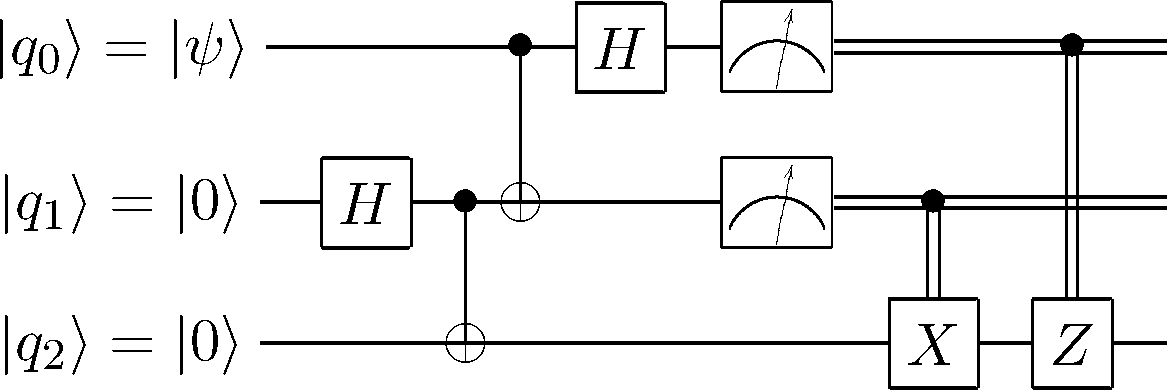
\includegraphics[height=2cm]{teleport.eps}
\caption{Circuit diagram for quantum teleportation.}
\end{figure}

\section*{Alegbraic verification}

Let $\ket{\psi} = a \ket{0} + b \ket{1}$ be the initial state of $q_0$.
The initial state of the register is

\begin{equation}
\ket{\psi} \tensor \ket{0} \tensor \ket{0} =
a \ket{000} + b \ket{100}.
\end{equation}

We prepare the two ancillary qubits $q_1$ and $q_2$ as an EPR pair by applying 
a Hadamard gate to $q_1$, then applying a CNOT gate to $q_2$ controlled
by $q_1$. The result is

\begin{equation}
	\ket{\psi} \tensor \frac1{\sqrt2} \left( \ket{00} + \ket{11} \right)
  = \frac1{\sqrt2} \left(a\ket{000} + a\ket{011} + b\ket{100} + b\ket{111}\right).
\end{equation}

The Bell measurement can be split into three steps:
\begin{enumerate}
	\item Apply a CNOT gate to $q_1$ controlled by $q_0$.
	\item Apply a Hadamard gate to $q_0$.
	\item Measure $q_0$ and $q_1$, yielding two classical bits $b_0$ and $b_1$.
\end{enumerate}

Applying the CNOT gate yields
\begin{equation}
	\frac1{\sqrt2} \left( a\ket{000} + a\ket{011} + b\ket{110} + b\ket{101}\right).
\end{equation}

The Hadamard gate maps $\ket{0}$ to $(\ket{0}+\ket{1})/\sqrt{2}$
and $\ket{1}$ to $(\ket{0} - \ket{1})/\sqrt2$. So applying a Hadamard gate to $q_0$ yields

\begin{equation}
\frac12 \left( a\ket{000} + a\ket{100} + a\ket{011} + a\ket{111} +
               b\ket{010} - b\ket{110} + b\ket{001} - b\ket{101}\right).
\end{equation}

We perform a measurement of the first two qubits ($q_0$ and $q_1$), yielding two classical bits
($b_0$ and $b_1$). There are four possible outcomes, as shown in the following table.

\begin{center}
\begin{tabular}{|c|c|c|}
\hline
$b_0$ & $b_1$ & new state \\
\hline
0 & 0 & $a\ket{000} + b\ket{001}$ \\
0 & 1 & $a\ket{011} + b\ket{010}$ \\
1 & 0 & $a\ket{100} - b\ket{101}$ \\
1 & 1 & $a\ket{111} - b\ket{110}$ \\
\hline
\end{tabular}
\end{center}

Recall that the Pauli-X gate maps $a\ket{0} + b\ket{1}$ to $b\ket{0} + a\ket{1}$,
and the Pauli-Z gate maps $a\ket{0} + b\ket{1}$ to $a\ket{0} - b\ket{1}$.

If $(b_0, b_1) = (0, 0)$ then we do nothing.
\begin{align}
a\ket{000} + b\ket{001} 
&= \ket{00} \tensor (a\ket{0} + b\ket{1}) \\
&= \ket{00} \tensor \ket{\psi}
\end{align}

If $(b_0, b_1) = (0, 1)$ then we apply a Pauli-X gate to $q_2$.
\begin{align}
a\ket{011} + b\ket{010} 
	&\mapsto a\ket{010} + b\ket{011} \\
    &= \ket{01} \tensor \ket{\psi}
\end{align}

If $(b_0, b_1) = (1, 0)$ then we apply a Pauli-Z gate to $q_2$.
\begin{align}
	a\ket{100} - b\ket{101} 
		& \mapsto a\ket{100} + b\ket{101} \\
 		& = \ket{10} \tensor \ket{\psi}
\end{align}

If $(b_0, b_1) = (1, 1)$ then we apply a Pauli-X gate followed by a 
Pauli-Z gate to $q_2$.
\begin{align}
	a\ket{111} - b\ket{110} 
		&\mapsto a\ket{110} - b\ket{111} \\
		&\mapsto  a\ket{110} + b\ket{111} \\
		&= \ket{11} \tensor \ket{\psi}
\end{align}


\end{document}
